%  LaTeX support: latex@mdpi.com 
%  For support, please attach all files needed for compiling as well as the log file, and specify your operating system, LaTeX version, and LaTeX editor.

%=================================================================
\documentclass[aerospace,article,submit,moreauthors,pdftex]{Definitions/mdpi} 

% For posting an early version of this manuscript as a preprint, you may use "preprints" as the journal and change "submit" to "accept". The document class line would be, e.g., \documentclass[preprints,article,accept,moreauthors,pdftex]{mdpi}. This is especially recommended for submission to arXiv, where line numbers should be removed before posting. For preprints.org, the editorial staff will make this change immediately prior to posting.

%--------------------
% Class Options:
%--------------------
%----------
% journal
%----------
% Choose between the following MDPI journals:
% acoustics, actuators, addictions, admsci, adolescents, aerospace, agriculture, agriengineering, agronomy, ai, algorithms, allergies, analytica, animals, antibiotics, antibodies, antioxidants, appliedchem, applmech, applmicrobiol, applnano, applsci, arts, asi, atmosphere, atoms, audiolres, automation, axioms, batteries, bdcc, behavsci, beverages, biochem, bioengineering, biologics, biology, biomechanics, biomedicines, biomedinformatics, biomimetics, biomolecules, biophysica, biosensors, biotech, birds, bloods, brainsci, buildings, businesses, cancers, carbon, cardiogenetics, catalysts, cells, ceramics, challenges, chemengineering, chemistry, chemosensors, chemproc, children, civileng, cleantechnol, climate, clinpract, clockssleep, cmd, coatings, colloids, compounds, computation, computers, condensedmatter, conservation, constrmater, cosmetics, crops, cryptography, crystals, curroncol, cyber, dairy, data, dentistry, dermato, dermatopathology, designs, diabetology, diagnostics, digital, disabilities, diseases, diversity, dna, drones, dynamics, earth, ebj, ecologies, econometrics, economies, education, ejihpe, electricity, electrochem, electronicmat, electronics, encyclopedia, endocrines, energies, eng, engproc, entropy, environments, environsciproc, epidemiologia, epigenomes, fermentation, fibers, fire, fishes, fluids, foods, forecasting, forensicsci, forests, fractalfract, fuels, futureinternet, futuretransp, futurepharmacol, futurephys, galaxies, games, gases, gastroent, gastrointestdisord, gels, genealogy, genes, geographies, geohazards, geomatics, geosciences, geotechnics, geriatrics, hazardousmatters, healthcare, hearts, hemato, heritage, highthroughput, histories, horticulturae, humanities, hydrogen, hydrology, hygiene, idr, ijerph, ijfs, ijgi, ijms, ijns, ijtm, ijtpp, immuno, informatics, information, infrastructures, inorganics, insects, instruments, inventions, iot, j, jcdd, jcm, jcp, jcs, jdb, jfb, jfmk, jimaging, jintelligence, jlpea, jmmp, jmp, jmse, jne, jnt, jof, joitmc, jor, journalmedia, jox, jpm, jrfm, jsan, jtaer, jzbg, kidney, land, languages, laws, life, liquids, literature, livers, logistics, lubricants, machines, macromol, magnetism, magnetochemistry, make, marinedrugs, materials, materproc, mathematics, mca, measurements, medicina, medicines, medsci, membranes, metabolites, metals, metrology, micro, microarrays, microbiolres, micromachines, microorganisms, minerals, mining, modelling, molbank, molecules, mps, mti, nanoenergyadv, nanomanufacturing, nanomaterials, ncrna, network, neuroglia, neurolint, neurosci, nitrogen, notspecified, nri, nursrep, nutrients, obesities, oceans, ohbm, onco, oncopathology, optics, oral, organics, osteology, oxygen, parasites, parasitologia, particles, pathogens, pathophysiology, pediatrrep, pharmaceuticals, pharmaceutics, pharmacy, philosophies, photochem, photonics, physchem, physics, physiolsci, plants, plasma, pollutants, polymers, polysaccharides, proceedings, processes, prosthesis, proteomes, psych, psychiatryint, publications, quantumrep, quaternary, qubs, radiation, reactions, recycling, regeneration, religions, remotesensing, reports, reprodmed, resources, risks, robotics, safety, sci, scipharm, sensors, separations, sexes, signals, sinusitis, smartcities, sna, societies, socsci, soilsystems, solids, sports, standards, stats, stresses, surfaces, surgeries, suschem, sustainability, symmetry, systems, taxonomy, technologies, telecom, textiles, thermo, tourismhosp, toxics, toxins, transplantology, traumas, tropicalmed, universe, urbansci, uro, vaccines, vehicles, vetsci, vibration, viruses, vision, water, wevj, women, world 

%---------
% article
%---------
% The default type of manuscript is "article", but can be replaced by: 
% abstract, addendum, article, book, bookreview, briefreport, casereport, comment, commentary, communication, conferenceproceedings, correction, conferencereport, entry, expressionofconcern, extendedabstract, datadescriptor, editorial, essay, erratum, hypothesis, interestingimage, obituary, opinion, projectreport, reply, retraction, review, perspective, protocol, shortnote, studyprotocol, systematicreview, supfile, technicalnote, viewpoint, guidelines, registeredreport, tutorial
% supfile = supplementary materials

%----------
% submit
%----------
% The class option "submit" will be changed to "accept" by the Editorial Office when the paper is accepted. This will only make changes to the frontpage (e.g., the logo of the journal will get visible), the headings, and the copyright information. Also, line numbering will be removed. Journal info and pagination for accepted papers will also be assigned by the Editorial Office.

%------------------
% moreauthors
%------------------
% If there is only one author the class option oneauthor should be used. Otherwise use the class option moreauthors.

%---------
% pdftex
%---------
% The option pdftex is for use with pdfLaTeX. If eps figures are used, remove the option pdftex and use LaTeX and dvi2pdf.

%=================================================================
% MDPI internal commands
\firstpage{1} 
\makeatletter 
\setcounter{page}{\@firstpage} 
\makeatother
\pubvolume{1}
\issuenum{1}
\articlenumber{0}
\pubyear{2021}
\copyrightyear{2020}
%\externaleditor{Academic Editor: Firstname Lastname} % For journal Automation, please change Academic Editor to "Communicated by"
\datereceived{} 
\dateaccepted{} 
\datepublished{} 
\hreflink{https://doi.org/} % If needed use \linebreak
%------------------------------------------------------------------
% The following line should be uncommented if the LaTeX file is uploaded to arXiv.org
%\pdfoutput=1

%=================================================================
% Add packages and commands here. The following packages are loaded in our class file: fontenc, inputenc, calc, indentfirst, fancyhdr, graphicx, epstopdf, lastpage, ifthen, lineno, float, amsmath, setspace, enumitem, mathpazo, booktabs, titlesec, etoolbox, tabto, xcolor, soul, multirow, microtype, tikz, totcount, changepage, paracol, attrib, upgreek, cleveref, amsthm, hyphenat, natbib, hyperref, footmisc, url, geometry, newfloat, caption

%=================================================================
%% Please use the following mathematics environments: Theorem, Lemma, Corollary, Proposition, Characterization, Property, Problem, Example, ExamplesandDefinitions, Hypothesis, Remark, Definition, Notation, Assumption
%% For proofs, please use the proof environment (the amsthm package is loaded by the MDPI class).

%=================================================================
% Full title of the paper (Capitalized)
\Title{Neural Network Prediction for Ice Shapes on Airfoils Using iceFoam Simulations}

% MDPI internal command: Title for citation in the left column
\TitleCitation{Neural Network Prediction for Ice Shapes on Airfoils Using iceFoam Simulations}

% Author Orchid ID: enter ID or remove command
\newcommand{\orcidauthorA}{0000-0001-5525-5180} % Add \orcidA{} behind the author's name
\newcommand{\orcidauthorB}{0000-0001-9568-7121} % Add \orcidA{} behind the author's name
\newcommand{\orcidauthorC}{0000-0002-7124-3945} % Add \orcidA{} behind the author's name
\newcommand{\orcidauthorD}{0000-0002-2052-3912} % Add \orcidA{} behind the author's name
%\newcommand{\orcidauthorB}{0000-0000-0000-000X} % Add \orcidB{} behind the author's name

% Authors, for the paper (add full first names)
\Author{Sergei Strijhak $^{1,2*}$ \orcidD{}, Daniil Ryazanov $^{1}$ \orcidB{},  Konstantin Koshelev $^{1,3}$ \orcidC{} and Aleksandr Ivanov $^{1,4}$\orcidA{} }

% MDPI internal command: Authors, for metadata in PDF
\AuthorNames{Sergei Strijhak, Daniil Ryazanov,  Konstantin Koshelev and Aleksandr Ivanov}

% MDPI internal command: Authors, for citation in the left column
\AuthorCitation{Strijhak, S.; Ryazanov, D.; Koshelev, K.; Ivanov, A.}
% If this is a Chicago style journal: Lastname, Firstname, Firstname Lastname, and Firstname Lastname.

% Affiliations / Addresses (Add [1] after \address if there is only one affiliation.)
\address{%
$^{1}$ \quad Ivannikov Institute for System Programming of the Russian Academy of Sciences, 109004, Moscow, Alexander Solzhenitsyn st., 25; s.strijhak@ispras.ru (S.S.), ryazanov@ispras.ru (D.R.). \\
$^{2}$ \quad Moscow Aviation Institute, 125993, Moscow, Volokolamskoe shosse, 4 \\
%; Sergei Strijhak s.strijhak@ispras.ru (S.S.) \\
$^{3}$ \quad Institute for Water and Environmental Problems, Siberian Branch of the Russian Academy of Sciences, 656038, Altai Krai, Barnaul, 1, Molodezhnaya St.; koshelevkb@mail.ru (K.B.)\\
$^{4}$ \quad Keldysh Institute of Applied Mathematics of the Russian Academy of Sciences, Miusskaya sq., 4, Moscow, 125047, Russia; av.ivanov@ispras.ru (A.I.)}


% Contact information of the corresponding author
\corres{Correspondence:  s.strijhak@ispras.ru (S.S.)}

% Current address and/or shared authorship
% The commands \thirdnote{} till \eighthnote{} are available for further notes

%\simplesumm{} % Simple summary

%\conference{} % An extended version of a conference paper

% Abstract (Do not insert blank lines, i.e. \$ 
\abstract{ 
This article gives the procedure and method for the ice accretion prediction for different airfoils using artificial neural networks (ANNs). A dataset for the neural network is based on the numerical experiment results with four airfoils (NACA0012, General Aviation, Business Jet, and Commercial Transport), which are obtained using the iceFoam solver. The input data for the neural networks includes airfoil and ice geometries, which are transformed into a set of parameters using a parabolic coordinate system and Fourier series expansion. Besides that the input features include physical parameters of flow (velocity, temperature, droplets diameter, liquid water content, time of ice accretion) and angle of attack. The novelties of this work are that the neural network dataset includes various airfoils and the data augmentation technique, which is all time slices combination. Several artificial neural networks (ANNs), fully connected networks (FCNNs), and convolutional networks (CNNs) are trained to airfoil ice shape prediction. Two different loss functions are considered. To improve models performance batch normalization and dropout layers are used. The most accurate result of ice shape prediction is received with CNN applying batch normalization and dropout layers to output neurons of each layer.}

% Keywords
\keyword{aircraft icing; airfoil; ice shape; CFD solver; simulation; dataset; loss function; neural network; CNN} 

% The fields PACS, MSC, and JEL may be left empty or commented out if not applicable
%\PACS{J0101}
%\MSC{}
%\JEL{}

%%%%%%%%%%%%%%%%%%%%%%%%%%%%%%%%%%%%%%%%%%
% Only for the journal Diversity
%\LSID{\url{http://}}

%%%%%%%%%%%%%%%%%%%%%%%%%%%%%%%%%%%%%%%%%%
% Only for the journal Applied Sciences:
%\featuredapplication{Authors are encouraged to provide a concise description of the specific application or a potential application of the work. This section is not mandatory.}
%%%%%%%%%%%%%%%%%%%%%%%%%%%%%%%%%%%%%%%%%%

%%%%%%%%%%%%%%%%%%%%%%%%%%%%%%%%%%%%%%%%%%
% Only for the journal Data:
%\dataset{DOI number or link to the deposited data set in cases where the data set is published or set to be published separately. If the data set is submitted and will be published as a supplement to this paper in the journal Data, this field will be filled by the editors of the journal. In this case, please make sure to submit the data set as a supplement when entering your manuscript into our manuscript editorial system.}

%\datasetlicense{license under which the data set is made available (CC0, CC-BY, CC-BY-SA, CC-BY-NC, etc.)}

%%%%%%%%%%%%%%%%%%%%%%%%%%%%%%%%%%%%%%%%%%
% Only for the journal Toxins
%\keycontribution{The breakthroughs or highlights of the manuscript. Authors can write one or two sentences to describe the most important part of the paper.}

%%%%%%%%%%%%%%%%%%%%%%%%%%%%%%%%%%%%%%%%%%
% Only for the journal Encyclopedia
%\encyclopediadef{Instead of the abstract}
%\entrylink{The Link to this entry published on the encyclopedia platform.}
%%%%%%%%%%%%%%%%%%%%%%%%%%%%%%%%%%%%%%%%%%

\begin{document}
%%%%%%%%%%%%%%%%%%%%%%%%%%%%%%%%%%%%%%%%%%
\setcounter{section}{0} %% Remove this when starting to work on the template.

%The order of the section titles is: Introduction, Materials and Methods, Results, Discussion, Conclusions for these journals: aerospace,algorithms,antibodies,antioxidants,atmosphere,axioms,biomedicines,carbon,crystals,designs,diagnostics,environments,fermentation,fluids,forests,fractalfract,informatics,information,inventions,jfmk,jrfm,lubricants,neonatalscreening,neuroglia,particles,pharmaceutics,polymers,processes,technologies,viruses,vision

\section{Introduction}

The study of the ice accretion is an important process for different aspects of people’s life, management of technical transportation and energy devices such as aircraft, helicopters, Unmanned Aircraft Systems, wind turbines, power electrical lines. 

The mass of growing ice can reach critical values and become the reason for the various technical problems or disasters. 
The ice thickness on the electric wires can reach dimensions comparable to the characteristic size or cable diameter, significantly weighting the wires, which can lead to wire breakage and metal supports breakage. For example, in November 2020 the power lines were cut off in a large Russian city Vladivostok under the weight of ice, trees and engineering structures were toppled. The cable-stayed bridge on Russky Island was in disrepair. As a result of this incident, about one hundred thousand residents of the Primorsky Territory of the Russian Federation were left without a power supply. Another example happened in October 2021 the hurricane wind and a blizzard brought down several substations in the north of Sakhalin at once. Bad weather disrupted the regular operation of the Okhinskaya Power Electrical station. The reason was the fall of the supports, overlap, and icing of the wires due to the stormy wind.  

Ice accretion on aircraft wing and helicopter rotor blades impairs its aerodynamic performance, which can lead to an aircraft crash. A detailed analysis of different aircraft crashes was presented in \cite{CaoTanWu2018}. One of the recent aircraft accidents due to icing in Russia in the case of An-148 aircraft of Russian Saratov Airlines, which was flying from Moscow to Orsk (Orenburg region), crashed on February 11, 2018, a few minutes after takeoff from Moscow's Domodedovo airport. The Interstate Aviation Committee noted \cite{IAC2018} that the problems could have been caused by icing of the sensors of the total pressure receivers, which measure the aircraft velocity.    
 
Currently, research projects on aircraft icing are underway in the USA, Europe, Canada, Japan, Russian Federation to develop the concept of new models of regional and supersonic passenger aircraft. The most famous projects are Aerion AS2, SpikeAero-space, Low Sonic Boom Configuration. Such an aircraft should be designed based on flight safety requirements, including those in difficult climatic conditions of the northern territories. The issues of studying the processes of formation of various forms of ice (rime, mixed, glaze, ridge) on different airfoils, changes in aerodynamic coefficients using experiment and mathematical modeling are relevant. The physical parameters of flow with water droplets up to 40 {\textmu}m in diameter are defined in Aviation Rules, Application C of Part 25 \cite{AP25} (Russia) or in FAA report \cite{FAA} (USA).

A detailed overview of the topic with aircraft icing is given in the following scientific works \cite{GentDartCansdale2000,CebeciKafyeke2003,LynchKhodadoust2001,CaoTanWu2018,YamazakiJemcovSakaue2021}.There are different approaches to the study of the ice accretion process (experimental, field, mathematical modeling with special codes, Machine Learning and Neural Networks). Some research teams have used approaches with Computational Fluid Dynamics (CFD) codes and artificial neural networks. The different numerical solvers for the ice accretion process have been developed since 1980. 

Among these codes are LEWICE, CANICE, AEROMSICE-2D, PoliMICE, NSCODE-ICE, ICECREMO, FENSAP-ICE, CLORNS, IGLOO2D. 

The research teams from different organizations develop their codes for ice accretion modeling: Beijing University of Aeronautics and Astronautics, China \cite{CaoHuangYin2016}, Nanjing University of Aeronautics and Astronautics, China \cite{WangZhaoZhu2018}, Politechnico di Milano, Italy \cite{Gori2015,ArizmendiBellosta2019}, Polytechnical Montreal University, Canada \cite{PenaHoarauLaurendeau2016}, University of Nottingham, UK \cite{JanjuaTurnbullHibberdChoi2018}, MCGill University, Canada \cite{BeaugendreMorencyHabashi2005}, 
%[Beaugendre, H., Morency, F., and Habashi, W. G., “Development of a Second Generation In-Flight Icing Simulation Code,” Journal of Fluids Engineering, Vol. 128, No. 2, 2006, pp. 378–387.].
ONERA, France \cite{TrontinVilledieu2017}.
%[Trontin, P., Kontogiannis, A., Blanchard, G., and Villedieu, P., “Description and assessment of the new ONERA 2D icing suite IGLOO2D,” 9th AIAA Atmospheric and Space Environments Conference--AVIATION 2017 DENVER, USA, AIAA 2017-3417, 2017, doi:10.2514/6.2017-3417.]

Over the past 10 years, a large number of articles have been published that are devoted to the application of machine learning methods, deep neural networks in the field of fluid dynamics and calculating aerohydrodynamic coefficients, and terms in the original equations reflecting conservation laws \cite{DuraisamyIaccarinoXiao2019}. Among them are the aerodynamic drag and lift coefficients \cite{zhang2018application}, the heat transfer coefficient, the induced mixing efficiency in stratified flows 
\cite{SalehipourPeltier2019}, the coefficients in engineering turbulence models \cite{ParishDuraisamy2016}, the Reynolds stress tensor 
\cite{LingKurzawskiTempleton2016}, turbulent scalar flux 
\cite{MilaniLingEaton2020},  the rate of physical and chemical reactions \cite{Lapeyre2019}. 

Previously, studies for research of ice accretion process were carried out using computational fluid dynamics and neural networks to simulate the ice formation process on the airfoils. A study was carried out of two architectures of neural networks that are best suited for this task \cite{OgretimHuebschShinn2006}:
\begin{itemize}
    \item a multilayer neural network with a learning algorithm using the back propagation of an error;
    \item a network of radial-basis functions.
\end{itemize}

To study the change in the airfoil shape during icing in 
\cite{ChangLengWuThompson2016}, an algorithm was used that involved two conformal mappings, namely, the investigated airfoil into a parabolic coordinate system and the Prandtl transposition to transform clean airfoil into a straight line. In this case, the shape of the frozen ice was presented as a perturbation of this line. The shape of the disturbance was set by the Fourier series or using wavelet functions \cite{ChangLengWuThompson2016}. The number of coefficients in the expansion and their values were the objects of prediction of the neural network.
The following parameters were used as input parameters for the neural network: 
\begin{itemize}
    \item atmospheric conditions (temperature $T$ and pressure $p$), 
    \item flight parameters (velocity $\vec U$), 
    \item droplet diameter $d$, 
    \item density or water content of drops, 
    \item drop time or time ice accretion $t$.
\end{itemize}

The results of the NASA experiment were used for validation. CFD simulations were performed using the NASA LEWICE package \cite{Wright2002}.

When studying the coefficients of the function approximating the shape of frozen ice, it was taken into account that their number should not greatly exceed the number of input parameters, otherwise the training time of the neural network would increase and the accuracy of the predicted results would decrease. The architecture of the neural network, which is based on dense neural network and it has one hidden layer, also provided a statistical inference of the relative significance of the input parameters in training.

The work \cite{ZhouGauger2019} considered the blade of the Sikorsky SC2110 helicopter. Using the PoliMIce library, the flows under icing conditions were calculated for different liquid water content (LWC) water conditions and median volume diameter (MVD) droplet sizes for 101 cases of airfoil. The data for the calculation were selected based on the data of the flight experiment. 

Deep Neural Network, Bayesian Neural Network together with CFD calculation results in SU2 code together with Ffowcs-Williams-Hawkings acoustic analogy to calculate far-field acoustic noise spectrum were used to calculate six aerodynamic coefficients (three coefficients for force, three coefficients for torque) 
%[5.	Beckett Y. Zhou, Nicolas R. Gauger et al. Towards a Real-Time In-Flight Ice Detection System via Computational Aeroacoustics and Bayesian Neural Networks. AIAA/ISSMO Multidisciplinary Analysis and Optimization at the AVIATION Forum, Dallas, Texas, 2019. 1-15 pp.]
\cite{ZhouGauger2019}. 
Based on the results of the performed comparative analysis, it can be concluded that the finite volume method is more preferable, since the basic equations reflecting the conservation laws are written in integral form. This method works effectively with structured and unstructured meshes.

The authors of \cite{LiQinHePaoli2020} introduced a purely data-driven approach to find the complex pattern between different flight conditions and aircraft icing severity prediction. The Extreme Gradient Boosting Supervised Learning (XGBoost) algorithm has been applied to create a prediction framework that makes a prediction based on any set of observations.

The input flight conditions for the proposed prediction framework are liquid water content, droplet diameter and exposure time. The proposed approach was demonstrated in three cases: maximum ice thickness prediction, icing area prediction and icing severity level evaluation.

Modeling a turbulent fluid flow around aircraft, taking into account the formation of ice of various shapes in a 3D setting, is an expensive computational procedure, especially when it is necessary to perform parametric studies. Approaches based on approximation with a decrease in the dimension of the system under study referred to as the methods of dimension reduction by means of Proper Orthogonal Decomposition (POD) are a good alternative for reducing computer time. 

Reduced Order Modeling (ROM) -- the approach uses the results or labeled snapshots obtained under specified conditions to construct basis vectors (modes) that reliably reproduce the main features of the flow. A linear combination of these modes can be used to obtain new solutions when specifying new input parameters that differ from previously obtained solutions (labeled snapshots). To obtain a system of reduced dimension, various methods can be used, including the POD 
\cite{ZhanHabashiFossati2015,ZhanHabashiFossati2016}.

In this approach, a global POD and a local POD can be used. Global POD uses all available solutions or labeled snapshots. In the case of icing simulation, different forms of ice are possible (rime ice -- loose ice, glaze ice -- smooth ice) when the initial parameters change. For external aerodynamics problems, different flow regimes are possible (shock waves, flow separation) when the Mach number changes for subsonic and transonic flow modes. 

The local POD method handles different physical characteristics in different ways. The local approach requires dividing the solution space into separate subdomains, each of which ideally contains solutions characterized by similar or sufficiently close physical structures. With solutions from each solution cluster, POD's linear approach allows for a generic solution using multiple modes. In several papers, the k-means algorithm, one of the machine learning methods, has been used to develop the local POD method.

As a rule, a software implementation of libraries for machine learning is done in Python programming language, using numerical libraries and the open frameworks such as Keras, scikit-learn, PyTorch, TensorFlow \cite{TensorFlow}.

The aim of this research work is specific library development for airfoil ice shape prediction based on the different models of neural networks. The main advantage of the library is to reduce computational costs of ice shape prediction using CFD packages.  

The main part of this paper has the following structure. Section~\ref{sec:mathematical-model} contains a description of the mathematical model for ice accretion simulation. Section~\ref{sec:Problemdefinition} describes the Definition of the problem for 2D airfoil. Section~\ref{sec:materialsAndMethods} describes Materials and Methods. Section~\ref{sec:results} contains the results of simulations with neural networks. Section~\ref{sec:discuss} contains Discussion. Section~\ref{sec:Conclus} concludes the paper.

%%%%%%%%%%%%%%%%%%%%%%%%%
%%%%%%%%%%%%%%%%%%%%%%%%%
%%%%%%%%%%%%%%%%%%%%%%%%%

\section{Mathematical model for ice accretion simulation}\label{sec:mathematical-model}

The mathematical models for ice accretion may include Euler-Euler, Euler-Lagrangian models,hybrid method with panel and integral Boundary Layer methods. To calculate the ice shape the iceFoam CFD solver is used which was developed in ISP RAS, and which is based on Euler-Lagrangian method, SWIM model for ice and fluid film simulation. \cite{KoshelevMelnikovaStrijhak2020}
%[Koshelev K.B., Melnikova V.G. Strijhak S.V. Development of iceFom solver for modeling ice accretion. Trudy ISP RAN/Proc. ISP RAS, vol. 1, issue 2, 2019. pp. 15-19 (in Russian).].

The iceFoam solver is being developed on the basis of the OpenFOAM package \cite{OpenFoam}. To describe the gas-droplet medium, the Euler-Lagrange model is used, which is based on a system of continuity, momentum, and energy equations, and the finite volume method for solving the initial  \cite{WellerTaborJasakFureby1998}. 

The iceFoam solver uses the PIMPLE algorithm for solving the velocity and pressure equations. When the gas-droplet flow interacts with the irregularities and the roughness of the solid surface of the body, an ice film and a liquid water film may appear and grow. 

This approach requires a separate unstructured mesh for the thin film area. As for the particles, the right-hand side of the equations for mass and energy contains source terms that characterize the processes of particles melting, splashing, convective heat transfer. The ice accretion leads to a change in the initial shape of the body. The boundary of the body moves in space along the normal. 

At the same time, it is necessary to ensure the simultaneous movement of borders for two different grids in the calculation program and recalculation of the position of grid nodes using the solution of the Laplace equation. To characterize the ability of the curved surface of the body to capture liquid drops, the water collection efficiency coefficient $\beta$ is used, and to describe thermal processes, the coefficient of heat transfer is applied.

The medium under consideration is a non-reacting equilibrium mixture of gases with a total temperature $T$, density $\rho$, and partial pressures $p_i$ for various components of the mixture.

In the framework of the selected mixture approximation, it is assumed that the mass, momentum and energy of the entire flow is transferred by the 	mass-averaged velocity $\vec{U}$ and the mass fraction of the mixture components of the flow incident on the body under study does not change with time.

The mutual motion of the mixture components is taken into account in the diffusion approximation. The effect of the dispersed phase on the continuous one is introduced as additional terms in the equations.

The mass conservation equation for the mixture:

\begin{equation}
    \frac{\partial\rho}{\partial t} + \nabla \cdot (\vec{U}\rho) = \dot{\rho_{v}},
\end{equation}

The momentum balance equation for the mixture:

\begin{equation}
     \frac{\partial\rho\vec{U}}{\partial t} + \nabla \cdot \left( \vec{U}\rho\vec{U} \right) + \sum_{i}^{}{\rho_{i}^{0}\vec{W_{i}}\vec{W_{i}}} = \dot{\rho_{v}}\vec{U_{v}} + \nabla \cdot \widehat{\sigma} - \nabla p.  %+\rho\vec{g} .    
\end{equation}

The energy balance equation with specific enthalpy for the mixture:

\begin{multline}
    \frac{\partial\rho h}{\partial t} + \nabla \cdot \left( \vec{U}\rho h \right) + \frac{\partial\rho K}{\partial t}  + \nabla \cdot \left( \vec{U}\rho K \right) +  \sum_{i}^{}{\nabla \cdot \vec{W_{i}}\rho_{i}^{0}e_{i}}  - \frac{\partial\ p}{\partial t}  = \\
    =  - \nabla \cdot (\widehat{\sigma} \cdot \vec{U}) - \nabla \cdot \vec{q} + \dot{\rho_{v}}e_{v}, 
\end{multline}

Where $\rho$ is the density of the mixture, 
$\rho_{i}^{0}$ is the density of the i-th component,
$\dot{\rho_{v}}$ is a source term describing the mass transfer between the gas and droplet phases, $\vec{W_{i}}$ is the relative speed, $\dot{\rho_{v}}\vec{U_{v}}$ is the exchange of momentum between the environment and drops of particles, $p$ is the ambient pressure, 
% $\vec{g}$ -- the acceleration of gravity, 
$\widehat{\sigma} = \mu\left( \nabla\vec{U} + {(\nabla\vec{U})}^{T} \right) - \frac{2}{3}\mu I\nabla \cdot \vec{U}$ is the viscous stress tensor; $\mu$ is the coefficient of viscosity of the mixture, $I$) is the identity tensor, $e$ is the internal energy of the mixture, 
$h$ is the specific enthalpy of the mixture, $K$ is the turbulence kinetic energy, 
$\dot{\rho_{v}}e_{v}$ is the exchange of energy between the environment and drops the particles.

The heat flux vector is calculated following Fourier's law $\vec{q} = - \lambda\nabla T$, where $\lambda$ -- the thermal conductivity of the mixture: 
$$
\quad C_{p} = \left( \frac{\partial h}{\partial T} \right)_{p}, 
\quad \nabla T = \frac{\nabla h}{C_{p}}.
$$

The specific enthalpy of a mixture is the weighted sum of the enthalpies of its components: 
$h = \sum_{i}^{}{Y_{i}h_{i}}$, where $Y_{i} = \dfrac{\rho_{i}^{0}}{\rho}$ is the mass fraction of the i-th component.

The mass balance equation of i-th component:
\begin{equation}
\label{eq:massBalance_i}
  \frac{\partial\rho Y_{i}}{\partial t} + \nabla \cdot \left( \vec{U}\rho Y_{i} \right) + \nabla \cdot \vec{W_{i}}\rho_{i}^{0} = 0.  
\end{equation}

The closing ratio for mass fractions of the mixture: $\sum_{i}^{}Y_{i} = 1$.

The average mass velocity $\vec{U}$ and relative velocities $\vec{W_{i}}$ are entered so that:

$$
\vec{U} = \frac{\sum_{i}^{}{\rho_{i}^{0}\vec{U_{i}}}}{\rho}, \;\;
\vec{W_{i}} = \vec{U} - \vec{U_{i}}, \;\;
\sum_{i}^{}{Y_{i}\vec{W_{i}}} = 0.
$$ 

To calculate the relative velocities of the gas components, the diffusion approximation is used:
$$
\rho_{i}^{0}\vec{W_{i}} = - D_{i}\nabla\rho_{i}^{0},
$$

where $D_{i}$ is the diffusion coefficient of the component: $D_{i} = \dfrac{\nu_{i}}{\text{Sc}}$ (the values of the number$\text{\ Sc}$ are calculated from the tables of medium properties depending on the temperature and composition of the mixture).

All components of the gaseous mixture are a perfect gas with a constant molar mass:
$$ 
p = \rho R \sum_{i}^{}\frac{Y_{i}}{M_{i}}T,
$$
where $R$ is the gas constant, $M_{i}$ is the molar mass of the i-th component.

The OpenFOAM particle cloud model sprayCloud is used as the base model. A cloud of spherical droplets-particles is determined by the position of its center of mass ${\vec{x}}_{p}$, the diameter of the incoming drops $D_{p}$, the speed of the drops ${\vec{U}}_{p}$, and the density of the substance $\rho_{p}$.

Then the mass of single particle:

$$m_{p} = \frac{1}{6}\rho_{p}\pi D_{p}^{3}.$$

The particles with similar parameters are represented by a cloud, since simulating all real droplet particles separately is expensive for computing resources. The clouds of particles do not interact with each other.

The trajectory of the particle cloud is determined by integrating the kinematics equation:

\begin{equation}
    \frac{{d\vec{x}}_{p}}{dt} = {\vec{U}}_{p}.    
\end{equation}

The particle velocity is determined from the solution of the force balance equation. The force acting on a particle is the sum of all the forces acting. Examples of such forces are the environmental drag force, gravity, buoyancy, and pressure force:

\begin{equation}
    m_{p}\frac{{d\vec{U}}_{p}}{dt} = \sum{\vec{F}}_{i} = {\vec{F}}_{D} + {\vec{F}}_{G} = \frac{3}{4}\frac{m_{p}\mu C_{D}\text{Re}_{p}}{\rho_{p}{D_{p}}^{2}}(\vec{U} - {\vec{U}}_{p}) + m_{p}\vec{g}(1 - \frac{\rho}{\rho_{p}}),    
\end{equation}
where ${\vec{F}}_{D}$ is the pressure force and ${\vec{F}}_{G}$ is the gravity force.

The $C_{D} \text{Re}_p$ complex is calculated depending on the selected model for calculating the drop drag coefficient using a function that depends on the Reynolds number of the particle $\text{Re}_{p}$.

There are available models: Putnam; Habashi; Prikhodko; Gent; Ochkov; Schiller-Neumann.

The Reynolds number for particle: $\text{Re}_{p} = \dfrac{\rho|\vec U - \vec U_{p}|D_{p}}{\mu}$.

The drop model also includes a drop mass balance equation:

\begin{equation}
    \frac{d m_{p}}{d t} = {\dot{m}}_{p} = 0,    
\end{equation}

and the heat balance equation for the drop:

\begin{equation}
    m_{p}C_{\text{pp}}\frac{dT_{p}}{dt} = Q_{T}    
\end{equation}

where $C_{\text{pp}}$ is the specific heat capacity at constant drop pressure;$\ T_{p}$ is the average volume temperature of the drop.

As a result of convective interaction with the main flow, the droplet jets take or give away part of the internal energy of the gas flow. Heat flow from the environment:

\begin{equation}
Q_{T} = \text{htc}_p \cdot S_{p} \cdot (T_{\text{sp}} - T),    
\end{equation}

where $S_{p} = \pi D_{p}^{2}$ is the surface area of the drop; $T$ is the ambient temperature.

The surface temperature drops $T_{\text{sp}}$:

\begin{equation}
    T_{\text{sp}} = \frac{2}{3}T_{p} + \frac{1}{3}T.    
\end{equation}

Heat transfer coefficient $\text{htc}$:

\begin{equation}
    \text{htc}_p = \frac{\text{Nu} \cdot \lambda}{D_{p}},    
\end{equation}

where $\lambda$ is the coefficient of thermal conductivity of the environment.

There are four models to choose from for calculation of heat transfer between the drop and the surrounding gas: Clift; Feng; Ranz-Marshall and Whitaker. The most widely used model is the Ranz-Marshall model, which uses coefficients to calculate the Nusselt number Nu for a spherical drop:

\begin{equation}
    \text{Nu} = 2 + 0.6\sqrt{\text{Re}_{p}} \cdot \sqrt[3]{\Pr}.    
\end{equation}

The Prandtl number of the gas $\Pr = \dfrac{c_{p}\mu}{\lambda} $ where $c_{p}$ is the specific heat capacity of the environment at constant pressure; $\mu$ is the dynamic viscosity of the surrounding gas.

To model film layers in OpenFOAM, one needs to select a special outer area of the grid from the aerodynamic region \cite{StrijhakKoshelevMelnikova2021}.
%[Strijhak S., Koshelev K, Melnikova V. Using a thermodynamic film model based on shallow water theory and a dynamic mesh model for the icing of 2D/3D bodies in the iceFoam solver simulation. International Conference on the Methods of Aerophysical Research, ICMAR 2020, Novosibirsk1 November 2020 до 7 November 2020]. 

All parameters of the thin film are calculated in this selected area of the grid. This grid area can be created using two OpenFOAM utilities. First, the \emph{topoSet} utility is used to extract all the cell faces of a section of the airfoil from the existing aerodynamic grid, and the extracted set of cell faces is used to extrude a new area of the grid using the \emph{extrudeToRegionMesh} utility. The \emph{extrudeToRegionMeshDict} dictionary sets parameters such as the set of cell faces to use, the number of layers, and the extrusion thickness.

To model the film layer, the so-called thin-film approximation is used, which means that the velocity normal to the grid on the wall is assumed to be zero. In addition, the tangential near-wall diffusion is considered insignificant compared to the normal near-wall diffusion.

\subsection{The SWIM model for liquid film}

Various models are used to simulate thermodynamic processes of icing on the surface. Among them are models: Messinger model \cite{MESSINGER}, Iterative Messinger Model \cite{ZHUFUSUNZHU2012}, and Myers model \cite{Myers2001}.
More details about thermodynamic models can be found in review \cite{Pierre2018}.

The SWIM is a Partial Differential Equation (PDE), developed for calculating the ice accretion process in its original form. It is represented by the following equations.

The flow in the wall film is calculated using the mass conservation equation:

\begin{equation}
    \frac{\partial\rho_{w}h_{w}}{\partial t} + \nabla \cdot \left( \rho_{w}h_{w} \vec u \right) = S_{imp} - S_{ice}    
\end{equation}

where $t$ is time, $\rho_{w}$ is the water density, $h_{w}$ is the thickness of the water film layer, $\vec u$ is the water film velocity, $S_{imp}$ is the mass added to the film layer due to particle collisions, and $S_{ice}$ is the mass change due to water solidification into ice.

The momentum balance equation in original SWIM model:

\begin{equation}
     \vec u = \frac{h_{w}}{2\mu_{w}} \vec \tau_{wall}  
\end{equation}

where $\mu_{w}$ is the dynamic viscosity of water, $\tau_{wall}$ is the air wall shear stress.

The energy balance equation:

\begin{multline}
    \frac{\partial\rho_{w}h_{w}H}{\partial t} + \nabla \cdot \left( \rho_{w}h_{w} \vec u H \right) = S_{imp}\frac{ \vec U_{imp}^{2}}{2} + Q_{c} - Q_{wall}+\\+ S_{imp}C_{w}\left( T_{imp} - T \right) - S_{ice}C_{ice}\left( T - T_{ref} \right) + S_{ice}L_{f} %???   
\end{multline}

where $H$ is the enthalpy of water, $U_{imp}$ is the impact droplet velocity,  $Q_{c}$ is the convective heat transfer, $Q_{wall}$ is the heat transfer to the airfoil surface, $C_{w}$ is the specific heat of water, $T_{imp}$ is the impinging droplets temperature, $T$ is the water film temperature, $C_{ice}$ is the specific heat of ice, $T_{ref}$ is the temperature of the triple point of water, $L_{f}$ is the fusion latent heat of ice.

The ice thickness $h_{ice}\ $ is determined by the formula:

\begin{equation}
    \rho_{ice}\frac{\partial h_{ice}}{\partial t} = S_{ice},    
\end{equation}
where $\rho_{ice}$ is the density of ice.

The system of equations has 5 unknowns $h_{w}, \vec u, T, S_{ice}, h_{ice}$ and cannot be solved directly. The main assumption of the SWIM model is that the film temperature is equal to the temperature of the triple point of water $(T = T_{ref})$. In this case, one can calculate all the unknowns, including the thickness of the water film and the thickness of the ice. In particular, the energy equation, assuming that the enthalpy is a function of temperature only $H_{f} = H\left( T_{ref} \right)$, takes the form:

\begin{equation}
    S_{ice} = \frac{S_{imp} H_{f} - S_{imp}\frac{\vec U_{imp}^{2}}{2}  - Q_{c} + Q_{wall} - S_{imp}C_{w}\left( T_{imp} - T_{ref} \right)}{H_{f} + L_{f}}   
\end{equation}

This paper introduces a modification of SWIM model, and the momentum balance equation has the form:

\begin{equation}
    \frac{\partial\rho_{w}h_{w} \vec u}{\partial t} + \nabla \cdot  \left( \rho_{w}h_{w} \vec u \vec u \right) = - h_{w}\nabla p + \vec S_{\rho \delta \vec U} + \vec \tau,
\end{equation}

where $p$ is the pressure, $\vec S_{\rho \delta \vec U}$ is the contribution from the falling drops, and $\tau$ is the stress from the forces acting on the film.

The heat transfer coefficient (htc) is very important parameter in the simulation of ice accretion for airfoils and wings. The predicted ice shape can be quite different from the actual scenario if the predicted htc is inaccurate.

In our model the heat transfer coefficient $\text{htc}$ is calculated using empirical formula, for which the spatial length scale $L$ must be specified. In the presence of turbulence, it is assumed that the effective values of the corresponding quantities are used. In what follows, the generally accepted variable notation is used. The local Reynolds and Prandtl numbers are calculated for the boundary cells.

\begin{equation}
    \text{Re } = \frac{\rho |\vec U| L}{ \mu},
    \label{eq:Re}
\end{equation}

\begin{equation}
    \text{Pr } = \frac{\mu C_p}{\lambda}.
    \label{eq:Pr}
\end{equation}

\begin{equation}
    \text{htc} =
    \begin{cases}
        0.664 \sqrt{\text{Re}} \sqrt[3]{\text{Pr}} \cdot \lambda /L, &\text{Re} < 5 \cdot 10^5; \\
        0.037 \sqrt{\text{Re}}^{0.8} \sqrt[3]{\text{Pr}}  \cdot \lambda /L,   &\text{Re} \geq 5 \cdot 10^5. \\
    \end{cases}
\end{equation}

The mathematical model is complemented by Reynolds-averaged Navier–Stokes (RANS) turbulence models $k\text{-}\varepsilon$, $k\text{-}\omega$ SST, Spalart-Allmaras \cite{wilcox2006turbulence}.

\subsection{The features of implementing the iceFoam solver in the OpenFOAM package 
\label{the-features-of-implementing-the-icefoam-solver-in-the-openfoam-package}}

\subsubsection{Implementing a dynamic grid}\label{implementing-a-dynamic-grid}

As part of the OpenFOAM package, it is necessary to implement the movement of grid nodes in two regions, i.e. in the area of the external gas-droplet flow and inside the film. The actual film grid in the OpenFOAM approach has only one cell in its thickness. The film cell size by thickness does not make physical sense and does not change when the calculated film thickness is changed. This is explained by the concept of the OpenFOAM package, which always solves 3D equations, even when they are described in 1D or 2D space in the original formulation. However, one should move the grid nodes according to the changing ice boundaries.

One of the proven algebraic methods for moving the grid is the bisector method. 

Since the nodes to change are located on the border between the two regions, it is necessary to rebuild the grid in the gas-droplet flow area. To do this, the standard OpenFOAM procedure based on solving the Laplace equation was used. As a boundary condition for it, the displacement of the ice boundary nodes is set. The solution gives the offset of all other nodes in the gas-droplet flow area.

\subsubsection{Different versions of iceFoam solver\label{sec:diff-icefoam-ver}}

3 versions of the iceFoam solver have been developed based on the Euler approach for the gas phase, the Lagrangian approach for modeling water droplets and a model of a water film on the surface of an airfoil over an ice layer. All three solvers use a water film and ice layer model that is linked to a shallow water model. 

The first version of the iceFoam solver is intended for initial estimation of icing spots of an arbitrary 3D airfoil. This solver fully uses all the capabilities of the Open-MPI technology for efficient parallel computations using the open source package OpenFOAM. 

The main limitation of this solver is the assumption that the thickness of the ice layer is sufficiently small and the change in the airfoil surface during icing can be neglected. The airfoil with ice and the ice-free airfoil are assumed to be the same. The developed extrudeToFilmCellDist utility is used to decompose the spatial region of the film. This utility makes it possible to ensure uniformity of domain decomposition in the gas domain and in the adjacent film. This version has no restrictions on the number of computational cores. 

The second version of the iceDyMFoam2 solver is designed to simulate icing with both rime ice and glaze ice, for which the ice surface often takes complex and bizarre shapes. In this version, the solver quite effectively allows to take into account the effect of changes in the airfoil surface during icing on the icing process itself. This solver requires the use of a structured mesh near the airfoil surface and the presence of only one spatial domain for the film and the adjacent Euler mesh. Computational experience has shown that this requirement limits the maximum number of computational cores. With a further increase in the number of computational cores used, the efficiency of parallel ones grows weakly or even decreases. 

To simplify the decomposition of the spatial gas domain, the addTwoLayersTo0 utility has been developed. This utility allows us to set the computational domain on the zero processor for the film and for two adjacent layers of the Eulerian grid of the gas phase of the flow. 

The third version of the iceDyMFoam3 solver also allows us to take into account the effect of changes in the airfoil surface during icing on the icing process itself. Like the first version, this solver fully uses all the capabilities of the Open-MPI parallel library technology to perform efficient parallel computations. Parallel implementation of the ice boundary required the use of low-level functions of the OpenFOAM package. In this case, there will necessarily be nodes that fall on the border of several domains. In the case of using the dynamic grid approach, it was necessary to collect information about nodes that are stored in several domains or on different computational cores. For such nodes, after local calculations within one domain, an operation was performed to determine the new position of the node. 

Next, averaging over all domains participating in the calculations of this node was performed. The averaged values of the position of nodes, which were recorded in more than one domain, were distributed back across all the necessary computational cores. Thus, the coincidence of moving nodes on different domains was ensured. For the case of icing with glaze ice, the third version of the iceDyMFoam3 solver is still inferior in its capabilities to the second version of the solver in terms of reliability. The extrudeToFilmCellDist utility is also used to decompose the spatial region of the film.

%%%%%%%%%%%%%%%%%%%%%%%%%
%%%%%%%%%%%%%%%%%%%%%%%%%
\section{Definition of the problem for 2D airfoil \label{sec:Problemdefinition}}

In this paper, initial boundary value problem for the case of flow around 2D airfoils is formulated. 

The numerical simulations for 2D airfoils (NACA0012, Business Jet, Commercial Transport, General Aviation) with different angle of attack were performed using domain with size $x=[-1;2]$ m, $z=[-1;1]$ m. Studies were conducted for case 421 using two different meshes. In the first variant, the number of cells was 16,000, 120 cells for a liquid film, and 30 cells in the area of ice growth, see Figure~\ref{fig:Mesh}. In the second variant the number of cells was 20,800, 180 cells for a liquid film and 60 cells in the area of ice growth. The results of calculating the thickness and shape of the ice turned out to be close, see Figure~\ref{fig:results421}. According to the results, (Figure~\ref{fig:results421}) the difference between the two meshes is insufficient, so the coarse one is used in this research due to lower computational costs. 

\begin{figure}[H]
    \centering
    \includegraphics[scale=0.115]{Figures/mesh421L0004.png}
    \caption{Mesh for simulation for 421 RUN case}
    \label{fig:Mesh}
\end{figure}

\begin{figure}[H]
    \centering
    \includegraphics[width=0.7\textwidth]{Figures/421-30-60.png}
    \caption{Results of ice simulation for 421 RUN case}
    \label{fig:results421}
\end{figure}

The numerical grid was built using the blockMesh, extrudeMesh and extrudeToRegionMesh OpenFOAM utilities \cite{OpenFoam}. The y+ average value for coarse mesh for the first near-wall cells was 5. 

The boundary conditions for velocity were the following: for inlet is Dirichlet boundary condition, for Outlet is Neumann boundary condition, for airfoil is no-slip boundary condition. For pressure the boundary conditions for inlet and outlet were calculated.

To approximate the terms in time the Euler scheme is used, to approximate the inviscid terms the first order upwind scheme is used, to approximate the viscous terms the second order linear corrected scheme is used. 

After discretization of the terms in the basic equations, the linear algebraic equations were solved numerically. The smoothSolver with smoother symGaussSeidel was used for calculation of velocity, the GAMG method with smoother GaussZeidel was used for calculation of pressure, the PBiCGStab method with preconditioner DILU was used for calculation of enthalpy.  

The initial position of spherical particles was set at the entrance to the computational domain, as well as the frequency with which the particles were introduced into the computational domain and the total mass of the particles. The temperature of the liquid particles was set equal to the ambient temperature. Thus, it was possible to calculate the LWC. The Reynolds equations and the high-Reynolds SST $k\text{-}\omega$ turbulence model with wall functions were used to describe the gas-droplet medium. The time step was chosen so that the local Courant number did not exceed 0.9.

The input parameters of the flow velocity correspond for Run case 421 (See Appendix \ref{sec:appA}).

Figure~\ref{fig:Mesh} shows the distribution of the thickness of the ice film over the surface and velocity fields on the dynamic mesh. Figure~\ref{fig:Decomposition} shows the domain decomposition for parallel simulations on high-performance cluster. Figure~\ref{fig:results421} presents the results of calculations of flow around NACA0012 for Run case 421 and comparison with experiment of NASA  \cite{SHINBOND1992,Addy2000IceAA}. Figure~\ref{fig:results425} presents the results of calculations of flow around NACA0012 for Run case 425 and comparison with experiment of NASA \cite{SHINBOND1992,Addy2000IceAA}. The value of length scale $L$ for calculation of htc in case Run 421 was set to 0.4.

\begin{figure}[H]
    \centering
    \includegraphics[scale=0.24]{Figures/421CellDist2.png}
    \caption{Results of domain decomposition for 421 RUN case}
    \label{fig:Decomposition}
\end{figure}

\begin{figure}[H]
    \centering
    \includegraphics[scale=0.37]{Figures/425.png}
    \caption{Results of ice simulation for 425 RUN case}
    \label{fig:results425}
\end{figure}

The dotted line shows the results of the NASA experiment, dashed line denotes the results obtained using the NASA LEWICE code, the color vector denotes the results obtained using iceDyMFoam3 solver. The time step was about $2 \cdot 10^{-4}$ seconds, and the number of particle packets was about 4,000. The 6 minutes of model icing time calculating  takes about 60 hours on a server with 12 computational cores. 

The number of particles in the pack was equal to 140,000. All the data for cases are mentioned in Table~\ref{tab:cases}, Appendix~\ref{sec:appA}. 

When the temperature changes, various forms of ice may form on airfoil as rime, glaze, mixed ices. One of the important requirements for the solver is the ability to run it in parallel mode. This allows us to significantly reduce the time spent on the simulation.

The numerical calculations of icing require significant resources of high-performance cluster. The use of neural networks can significantly reduce the use of expensive computer's time. The issues of choosing the optimal architecture of a neural network, the choice of input parameters and the required metrics are topical. 

%%%%%%%%%%%%%%%%%%%%%%%%%

%%%%%%%%%%%%%%%%%%%%%%%%%%%%%%%%%%%%%%%%%%
\section{Materials and Methods \label{sec:materialsAndMethods}}

\subsection{Generation of datasets}

Ice shape dataset was obtained for 4 different 2D airfoils (NACA0012, Business Jet, Commercial Transport, General Aviation). The geometry for airfoils is described in \cite{SHINBOND1992,Addy2000IceAA}, the description of considered cases one can see in Appendix~\ref{sec:appA}. %Harold E. Addy, Jr. Ice Accretions and Icing Effects for Modern Airfoils. NASA /TP-2000-210031.].  
The final dataset includes the ice thickness which was represented by two coordinates x,y, time steps, and 6 physical parameters which determined the condition of ice accretion.

The shape of the ice on the airfoil can be approximate using a mathematical function. Further research is related to the analysis of this function and its representation using the Fourier transform. 

\subsection{Analysis of shape function \label{sec:Fourier}}

Parametrization of the airfoil shape and the ice formed on it is a difficult problem. The shapes of different airfoils are complex curves that cannot be parameterized with a single set of coefficients. On the other hand, the grid representation of geometry in the form of a set of points with coordinates $(x, y)$ also cannot be used as parameters, since, firstly, this set of parameters strongly depends on the choice of the grid and secondly the number of such parameters will grow rapidly with decreasing the size of the grid cell. To solve this problem, the approach implemented in \cite{OgretimHuebschShinn2006} was used. The main idea of this approach is to use the transformation of an airfoil shape into a function, which can then be expanded into a Fourier series. The Fourier coefficients will unambiguously determine the specified airfoil.

Let us briefly describe the process of transition from an airfoil to a set of Fourier coefficients.

As a result of the calculation, there is a set of ordered points that determine the state of the airfoil depending on the given moment in time $ t_i $: $(x_j (t_i), y_j (t_i)), j = \overline{1, N_{grid}}, i = \overline{1, M} $, where $ N_{grid} $ is the number of grid elements that define the airfoil geometry, and $ M $ is the number of time slices.

To transform an airfoil curve into a function, it is necessary to use a parabolic coordinate system. On the other hand, for the points of the investigated airfoils to fit better on the ground, it is necessary to scale them by dividing them by the leading edge radius ($ r_l $):
\begin{equation}
    \label{eq:xy_scale}
    x'_i = x_i/r_l - 0.5, \quad y'_i = y_i/r_l.
\end{equation}
The x-axis shift by 0.5 to the right is necessary so that the leading edge of the airfoil lies inside the parabola.

The $ r_l $ value is determined by the airfoil, however for a uniform conversion of all airfoils, the average value $ r_l = 0.03 c $ was used, where $ c $ is the chord length. All airfoils (except NACA0012) have a chord length of approximately 1 m, so the radius is $ r_l = 0.03 $ m. 

Then the transformation into the parabolic coordinate system $ (\xi, \eta) $ is done:
\begin{equation}
    \label{eq:ksi_eta}
    \xi_i = \mathrm{sgn}(y_i) \sqrt{x_i + \sqrt{x_i + y_i}}, \quad \eta_i = \sqrt{-x_i + \sqrt{x_i + y_i}}.
\end{equation}

Thus representing the airfoil as a function expressed by a set of points $ \eta = f (\xi) $, one can write out formulas for determining $ N $ coefficients of the Fourier series expansion on some segment $ [\xi_a, \xi_b] $, the length of which is $ L_{ab} = \xi_b - \xi_a $:
\begin{equation}
    \label{eq:fcoeffs}
    a_k = \frac{2}{L_{ab}} \int_{\xi_a}^{\xi_b} f(\xi) \cos \left( \frac{2 \pi k \xi}{L_{ab}}\right) d \xi, \quad
    b_k = \frac{2}{L_{ab}} \int_{\xi_a}^{\xi_b} f(\xi) \sin \left( \frac{2 \pi k \xi}{L_{ab}}\right) d \xi, \quad k = \overline{0,N}. 
\end{equation}
Note that these integrals are calculated numerically, for example, using the Simpson formula, and using the already given partition $ (\xi_i, \eta_i) $. This partition can be supplemented with intermediate points using interpolation to calculate the Fourier coefficients with large numbers since their integrands oscillate strongly.

Then, summing up the corresponding Fourier series, one can obtain an approximation of the function $ f (\xi) $:
\begin{equation}
    \label{eq:FSeries}
    \Tilde{f} (\xi) = \frac{a_0}{2} + \sum_{k = 1}^N \left( a_k \cos \left( \frac{2 \pi k \xi}{L_{ab}}\right) + b_k \sin \left( \frac{2 \pi k \xi}{L_{ab}}\right) \right).
\end{equation}

It is important to note that the resulting expression (\ref{eq:FSeries}) is a function that allows to restore the shape of the airfoil at any point on the segment $ [\xi_a, \xi_b] $.

To predict the thickness of accumulated ice, it is not necessary to consider the entire airfoil. For the studied airfoils, the change in the function representing the displacement of the geometry due to the ice accretion is localized on the segment $[- 4;4]$ therefore next it is assumed that
$$
\xi_a = -4, \quad \xi_b = 4, \quad L_{ab} = 8. 
$$

\subsection{Augmentation of data}

One of the novelties of this work is training a neural network on various airfoils. Due to this fact it is necessary to include in the set of training parameters the geometry of the original airfoil, which has the form of a set of Fourier coefficients $ \{a_k^{in}, b_k^{in} \} $. It is not necessary to look for the result in the form of Fourier coefficients required to restore the geometry. It is enough to get the coefficients representing the geometry change $ \{\Tilde {a}_k^{out}, \Tilde {b}_k^{out} \} $, then the resulting airfoil shape can be restored by adding the input and output coefficients:
\begin{equation}
\label{eq:coeffsOut}
    \{a_k^{res},b_k^{res}\} = \{a_k^{in},b_k^{in}\} + \{\Tilde{a}_k^{out},\Tilde{b}_k^{out}\}, \quad k = \overline{1,N}.
\end{equation}

Another novelty is the use of all time slices as input to learning. The main goal of forecasting using machine learning is to obtain the final ice build-up on a clean airfoil under given external conditions at time $ t $. Since the source of data in this study is a numerical calculation, instead of a clean airfoil, one can consider every intermediate time moment as the initial state. This approach allows us to significantly increase the amount of data for training a neural network.

Suppose the calculation case contains $ M $ time slices: $ t_0 = 0, t_1, t_2, \dots, t_{M-1} $. Then for the initial moment of time, it is possible to choose $M -1$ the final state, which can be obtained depending on the value of the icing time. For the moment $t_1$ such resulting states will be $ M - 2 $, etc. The sum of all obtained pairs in the form $ \{t_i, t_j \} $ can be obtained as the sum of an arithmetic progression:
\begin{equation}
    \label{eq:pairsnum}
    S(M) = \frac{M (M - 1)}{2}. 
\end{equation}

\subsection{Features definition}

Besides the main icing parameters: velocity $\vec U$, temperature $T$, liquid water content $LWC$, the droplets diameter $MVD$, time of icing accretion $t$ and angle of attack $AOA$, the airfoil shape is suggested to be used as input feature. This allows us to account for the airfoil form changing and to predict ice shape for different airfoils. According to Section~\ref{sec:Fourier} the airfoil shape is represented by $2N + 1$ coefficients. To find a better value for $N$ many numerical experiments were conducted. It was shown that on the one hand, if $N \leq 10$, the function of ice shape will have oscillations due to lack of high-frequency terms in (\ref{eq:FSeries}). On the other hand, the contribution of high-frequency terms is significantly decreasing with increasing $N$ due to the Fourier coefficients properties. In this work the $N = 20$ as optimal value for models performance. Therefore the overall number of the input parameters is $47$.

The output parameters for prediction are the $2N +1$ Fourier coefficients, which represent the form of the airfoil with accumulated ice. 

\subsection{Metric definitions \label{sec:metric}}

There are two different metrics for error estimation. The first one is the Mean Squared Error (MSE)
\begin{equation}
    err_{\text{MSE}} = \frac{1}{N_f} \sum_{k = 1}^{N_f} \left( c^p_{k} - c^t_{k} \right)^2, \quad N_f = 2N + 1,
    \label{eq:MSE}
\end{equation}
where $c_k$ denotes both sine $b_k$ and cosine $a_k$ Fourier coefficients from (\ref{eq:fcoeffs}). Hereinafter upper indexes $p$ and $t$ mean \textit{prediction} and \textit{target}, respectively. An $err_{\text{MSE}}$ is applied directly to the Fourier coefficients, unlike the error $\Tilde{err}$ which is usually used to estimate ice shape prediction error \cite{OgretimHuebschShinn2006,ChangLengWuThompson2016} and applied to the function deduced from the Fourier series (\ref{eq:FSeries}):
\begin{equation}
    \Tilde{err} = \frac{\int_{\xi_a}^{\xi_b} | f^p - f^t | dx}{\int_{\xi_a}^{\xi_b} f^t dx}.
    \label{eq:oldIoU}
\end{equation}

In this paper the intersection over union (IoU) error $ err_{\text{IoU}}$ is suggested, which is the ratio of the ice shape difference area and the total area of the predicted and target ice shapes:
%, see Figure~\ref{fig:IoU}:
\begin{equation}
    err_{\text{IoU}} = \frac{\int_{\xi_a}^{\xi_b} | f^p - f^t | dx}{2 \int_{\xi_a}^{\xi_b} (|f^p| + |f^t|) dx - \int_{\xi_a}^{\xi_b}|f^p  -  f^t| dx}
    \label{eq:IoU}
\end{equation}

\subsection{Neural Networks \label{sec:NN}}

The development of ice on airfoils using models with two different architectures of neural networks FCNN and CNN is studied. The choice of such architectures was based on the classical concepts of neural networks. The training procedure is the optimization of the coefficients of connections between neurons. The training algorithm is various modifications of the gradient descent are usually used to train models. According to the division of the complete dataset into training, validation, and test sets, training was carried out in batches, each batch containing 32 examples from the training set. Splitting into batches is needed to stabilize training.

A fully connected neural network (FCNN) is the simplest concept of architecture. Each neuron connects with each neuron in subsequent layer, see Figure~\ref{fig:denseScheme}. Input and output layers are determined by the problem. The number of hidden layers and neurons on them is not defined and can be arbitrary. FCNN has a disadvantage in the curse of dimension, even a small increase in the number of layers and neurons leads to a significant increase in learning parameters. 

\begin{figure}[H]
\centering
\includegraphics[width=0.5\textwidth]{Figures/denseScheme.pdf}
\caption{FCNN architecture.\label{fig:denseScheme}}
\end{figure}  

In addition to the fully connected neural network, Convolutional Neural Networks were used. CNN is very popular today to use in image analysis for unsolved problems in medicine and in satellite imagery analysis for rapid response to natural hazards (Floods, Landslide, Water Pollution) on Earth  \cite{RonnebergerFischerBrox2015,BullockBofarull2019,NemniBullockBelabbesBromley2020}.

%

%[1. Ronneberger, O.; Fischer, P.; Brox, T. U-Net: Convolutional Networks for Biomedical Image Segmentation. In Medical Image Computing and Computer-Assisted Intervention; Navab N., Hornegger J., Wells W., Frangi A., Eds; MICCAI 2015. Lecture Notes in Computer Science; Springer: Cham, Switzerland, 2015, Volume 9351.  
%2. Bullock, J.; Cuesta-Lázaro, C.; Quera-Bofarull, A. XNet: A convolutional neural network (CNN) implementation for medical x-ray image segmentation suitable for small datasets. In Medical Imaging 2019: Biomedical Applications in Molecular, Structural, and Functional Imaging; Gimi, B., Krol, A., Eds.; International Society for Optics and Photonics: Bellingham, WA, USA, 2019; Volume 10953, pp. 453–463. 
%3. Edoardo Nemni , Joseph Bullock, Samir Belabbes and Lars Bromley. Fully Convolutional Neural Network for Rapid Flood Segmentation in Synthetic Aperture Radar Imagery. Remote Sens. 2020, 12, 2532; doi:10.3390/rs12162532.]

Convolutional layers have significantly fewer training parameters, which gives finer possibilities for determining the complexity of the model. Filters are considered to generalize spatial structures, Figure \ref{fig:cnn}. The use of convolutional neural networks in this task is due to the hypothesis of the influence of ice accretion on each other during their formation.

\begin{figure}[H]
\centering
\includegraphics[width=0.5\textwidth]{Figures/CNNScheme.eps}
\caption{CNN architecture.\label{fig:cnn}}
\end{figure}  

To improve the prediction performance, several neural networks have been tested and their modifications. Besides using two types of neural networks FCNN and CNN and applying them with two different loss functions, see Section~\ref{sec:metric}, two additional methodologies: batch normalization and neurons dropout are used. Thus there are 12 NN:  FCNN$_{\text{IoU}}$, FCNN$_{\text{IoU}}^{B}$, FCNN$_{\text{IoU}}^{B,D}$, FCNN$_{\text{MSE}}$, FCNN$_{\text{MSE}}^{B}$, FCNN$_{\text{MSE}}^{B,D}$, see Table~\ref{tab:FCNN} and CNN$_{\text{IoU}}$, CNN$_{\text{IoU}}^{B}$, CNN$_{\text{IoU}}^{B,D}$, CNN$_{\text{MSE}}$, CNN$_{\text{MSE}}^{B}$, CNN$_{\text{MSE}}^{B,D}$, see Table~\ref{tab:CNN}. Here lower index means error type (MSE and IoU for mean squared error and intersection over union respectively), upper index denotes whether the model applies batch normalization layer to every output neurons ($B$) or drops out $50\%$ of output neurons ($D$).

\begin{table}[]
    \caption{Architecture for different FCNN models}
    \centering
    \begin{tabular}{c c c c c c}
    \toprule
	& \textbf{Output}	& \textbf{Number } & &  & \\
    \textbf{Layer type}	& 	& \textbf{of trainable } & \textbf{FCNN} & \textbf{FCNN$^B$} & \textbf{FCNN$^{B,D}$}\\
   	& \textbf{shape}	& \textbf{parameters} &  &  & \\
	\midrule
        Dense                       & 64 & 3,136 & contains & contains & contains\\
        Batch Normalisation         & 64 & 256 & - & contains & contains\\
        Activation (ReLu)           & 64 & 0 & - & contains & contains\\
        Dropout 50\% (ReLu)         & 64 & 0 & - & - & contains\\
        Dense                       & 128 & 8,320  & contains & contains & contains\\
        Batch Normalisation         & 128 & 512 & - & contains & contains\\
        Activation (ReLu)           & 128 & 0 & - & contains & contains\\
        Dropout 50\% (ReLu)         & 128 & 0 & - & - & contains\\
        Dense                       & 256 & 33,024 & contains & contains & contains\\
        Batch Normalisation         & 256 & 1024 & - & contains & contains\\
        Activation (ReLu)           & 256 & 0 & - & contains & contains\\
        Dropout 50\% (ReLu)         & 256 & 0 & - & - & contains\\
        Dense                       & 128 & 32,896 & contains & contains & contains\\
        Batch Normalisation         & 128 & 512 & - & contains & contains\\
        Activation (ReLu)           & 128 & 0 & - & contains & contains\\
        Dropout 50\% (ReLu)         & 128 & 0 & - & - & contains\\
        Dense                       & 64 & 8,256 & contains & contains & contains\\
        Batch Normalisation         & 64 & 256 & - & contains & contains\\
        Activation (ReLu)           & 64 & 0 & - & contains & contains\\
        Dropout 50\% (ReLu)         & 64 & 0 & - & - & contains\\
        Dense                       & 41 & 2,665 & contains & contains & contains\\
        \midrule
        Total parameters: & & & 88,393 & 89,673 & 89,673
    \end{tabular}
    \label{tab:FCNN}
\end{table}

\begin{table}[]
    \caption{Architecture for different CNN models}
    \centering
    \begin{tabular}{c c c c c c}
    \toprule
	& \textbf{Output}	& \textbf{Number } & &  & \\
    \textbf{Layer type}	& 	& \textbf{of trainable } & \textbf{CNN} & \textbf{CNN$^B$} & \textbf{CNN$^{B,D}$}\\
   	& \textbf{shape}	& \textbf{parameters} &  &  & \\
	\midrule
        Batch Normalisation         & 48 & 4 & contains & contains & contains\\
        Activation (ReLu)           & 48 & 0 & contains & contains & contains\\
        Convolution                 & $45 \times 32$ & 160 & contains & contains & contains\\
        Batch Normalisation         & $45 \times 32$ & 128 & - & contains & contains\\
        Activation (ReLu)           & $45 \times 32$ & 0 & - & contains & contains\\
        Dropout 50\% (ReLu)        & $45 \times 32$ & 0 & - & - & contains\\
        Convolution                 & $42 \times 32$ & 4,128 & contains & contains & contains\\
        Batch Normalisation         & $42 \times 32$ & 128 & - & contains & contains\\
        Activation (ReLu)           & $42 \times 32$ & 0 & - & contains & contains\\
        Dropout 50\% (ReLu)        & $42 \times 32$ & 0 & - & - & contains\\
        Convolution                 & $39 \times 32$ & 4,128 & contains & contains & contains\\
        Batch Normalisation         & $39 \times 32$ & 128 & - & contains & contains\\
        Activation (ReLu)           & $39 \times 32$ & 0 & - & contains & contains\\
        Dropout 50\% (ReLu)        & $39 \times 32$ & 0 & - & - & contains\\
        Convolution                 & $36 \times 32$ & 4,128 & contains & contains & contains\\
        Batch Normalisation         & $36 \times 32$ & 128 & - & contains & contains\\
        Activation (ReLu)           & $36 \times 32$ & 0 & - & contains & contains\\
        Dropout 50\% (ReLu)        & $36 \times 32$ & 0 & - & - & contains\\
        Convolution                 & $30 \times 32$ & 4,128 & contains & contains & contains\\
        Batch Normalisation         & $30 \times 32$ & 128 & - & contains & contains\\
        Activation (ReLu)           & $30 \times 32$ & 0 & - & contains & contains\\
        Dropout 50\% (ReLu)        & $30 \times 32$ & 0 & - & - & contains\\
        Convolution                 & $27 \times 32$ & 4,128 & contains & contains & contains\\
        Batch Normalisation         & $27 \times 32$ & 128 & - & contains & contains\\
        Activation (ReLu)           & $27 \times 32$ & 0 & - & contains & contains\\
        Dropout 50\% (ReLu)        & $27 \times 32$ & 0 & - & - & contains\\
        Convolution                 & $24 \times 32$ & 4,128 & contains & contains & contains\\
        Batch Normalisation         & $24 \times 32$ & 128 & - & contains & contains\\
        Activation (ReLu)           & $24 \times 32$ & 0 & - & contains & contains\\
        Dropout 50\% (ReLu)        & $24 \times 32$ & 0 & - & - & contains\\
        Pooling                     & $12 \times 32$ & 0 & contains & contains & contains\\
        Flatten                     & $384$ & 0 & contains & contains & contains\\
        Dense                       & 41 & 15,785 & contains & contains & contains\\
        \midrule
        Total parameters: & & & 44,543 & 45,355 & 45,355
    \end{tabular}
    \label{tab:CNN}
\end{table}

The main aim of model training is empirical risk minimization -- calibrating the coefficients of the model so as to minimize the average error on the training sample \cite{vapnik1992principles}. The first attempts to build approximation models based only on dense layers for FCNN or using filters and pooling layers for CNN led to strong overfitting. This is clear from the high spread of errors in the training and test samples (see results for FCNN$_{\text{IoU}}$, FCNN$_{\text{MSE}}$, CNN$_{\text{IoU}}$ and CNN$_{\text{MSE}}$, Figures~\ref{fig:losIoU} and \ref{fig:losMSE}). This NN don't give the desired performance. These results are due to a high variance of training data or excess model complexity. On the other hand, simplifying the model entails the other extreme is underfitting and results between these two architectures are unsatisfied.

Figures~\ref{fig:losIoU} and \ref{fig:losMSE} demonstrate the comparison of model performance for two metrics. To compare two sets of models the MAE error was computed, see Figure~\ref{fig:losMAE}.

To solve the overfitting problem one can use approaches such as batch normalisation or regularisation with dropout. The neural network design guidelines state that the batch normalization layer must follow the fully connected layer prior to activation \cite{ioffe2015batch}. 

In Figure~\ref{fig:losMAE} one can see that batch normalisation layers significantly improved results and decrease test error for IoU metric, but not for MSE. One of the possible reason for this is that MSE is an absolute error, while IoU is relative. That means that the model trains faster and there is overfitting even for models with batch normalization and dropout. 

The next modification of the NN is adding $D$ layers, which drop out 50\% of neurons. This models demonstrate the better performance, see Figure~\ref{fig:losMAE}.

\begin{figure}[H]
\includegraphics[width=0.6\textwidth]{Figures/losIoU.png}
\caption{Comparison of the losses in IoU metric for different neural networks modifications.\label{fig:losIoU}}
\end{figure} 

\begin{figure}[H]
\includegraphics[width=0.6\textwidth]{Figures/losMSE.png}
\caption{Comparison of the losses in MSE metric for different neural networks modifications.\label{fig:losMSE}}
\end{figure} 

\begin{figure}[H]
\includegraphics[width=0.6\textwidth]{Figures/losMAE.png}
\caption{Comparison of the losses in MAE metric for different neural networks modifications.\label{fig:losMAE}}
\end{figure} 

%%%%%%%%%%%%%%%%%%%%%%%%%%%%%%%%%%%%%%%%%%
\section{Results \label{sec:results}}

According to MAE metric, Figure~\ref{fig:losMAE}, one can see, that convolutional neural network with batch normalization and dropout layers demonstrates the best performance. Also the results in  Figure~\ref{fig:losMAE} demonstrates that there is almost no difference between metric IoU and MSE.   

To train the models the cases (see Table~\ref{tab:cases}) were randomly divided into three groups: 
\begin{itemize}
    \item Train: (15 cases) 421, 73195.02, 642, 645, 424, 128, 422, 423, 425, 214, 625, 622, 629, 632, 122;
    \item Validation: (3 cases): 129, 621, 124;
    \item Test: (4 cases): 407, 613, 222, 626.
\end{itemize}

The number of cases ratio for datasets is 68\%/14\%/18\% for Train/Validation/Test respectively. The total number of pairs in format $\{input,target\}$ is 147,679.


%[1.Reza Zadeh, Bharath Ramsundar. TensorFlow for Deep Learning: From Linear Regression to Reinforcement Learning. 2018. ISBN-13: 978-1491980453
%2. François Chollet . Deep Learning with Python . Second Edition. 2021. ISBN-13: 978-1617296864.] 

The results for FCNN$_{\text{IoU}}^{B,D}$ and FCNN$_{\text{IoU}}^{B,D}$ presented in Figure~\ref{fig:407}--\ref{fig:626}.

\begin{figure}[H]
\includegraphics[width=0.6\textwidth]{Figures/407.png}
\caption{Comparison of the NACA0012 407 case ice shape for the iceFoam, FCNN$_{\text{IoU}}^{B,D}$ and CNN$_{\text{IoU}}^{B,D}$.\label{fig:407}}
\end{figure} 
\begin{figure}[H]
\includegraphics[width=0.6\textwidth]{Figures/613.png}
\caption{Comparison of the GA 613 case ice shape for the iceFoam, FCNN$_{\text{IoU}}^{B,D}$ and CNN$_{\text{IoU}}^{B,D}$.\label{fig:613}}
\end{figure} 
\begin{figure}[H]
\includegraphics[width=0.6\textwidth]{Figures/222.png}
\caption{Comparison of the BJ 222 case ice shape for the iceFoam, FCNN$_{\text{IoU}}^{B,D}$ and CNN$_{\text{IoU}}^{B,D}$.\label{fig:222}}
\end{figure} 
\begin{figure}[H]
\includegraphics[width=0.6\textwidth]{Figures/626.png}
\caption{Comparison of the GA 626 case ice shape for the iceFoam, FCNN$_{\text{IoU}}^{B,D}$ and CNN$_{\text{IoU}}^{B,D}$.\label{fig:626}}
\end{figure} 

Figure~\ref{fig:EpochFig} demonstrates the dynamic of losses on the training and validation datasets over training epochs. 

\begin{figure}[H]
\includegraphics[width=0.6\textwidth]{Figures/EpochFig.png}
\caption{Loss per epoch for FCNN$_{\text{IoU}}^{B,D}$ and CNN$_{\text{IoU}}^{B,D}$.\label{fig:EpochFig}}
\end{figure} 

Compared to the CFD packages' computational time, which is from several hours to a few days, the neural network prediction process takes about 3--5 minutes, including time for training. 

The final result of the presented work is the specific library development for ice shape prediction using neural networks -- iceMPLNet.   

%%%%%%%%%%%%%%%%%%%%%%%%%%%%%%%%%%%%%%%%%%
\section{Discussion \label{sec:discuss}}

Our approach included some new features, like training a neural network on various airfoils, using of all time slices as input for learning.
Several neural networks with batch normalization and dropout layers are also used.The intersection over union (IoU) error $err_{\text{IoU}}$ is used, which is the ratio of the ice shape difference area and the total area of the predicted and target ice shapes.

Future research directions are to study the effects of icing on different parts of 3D aircraft wings. The future development of iceMPLNet is aimed to ice mass and main aerodynamic coefficients prediction. 

%%%%%%%%%%%%%%%%%%%%%%%%%%%%%%%%%%%%%%%%%%
\section{Conclusions \label{sec:Conclus}}

The iceFoam solver has been developed as part of the OpenFOAM package to simulate the process of airfoil icing. Its features are the use of the Euler-Lagrangian approach to describe the behavior of the gas-droplet flow, the possibility of using various models of the water film on the ice surface, a dynamic computational grid, and the possibility of using parallel calculations. The solver allows us to flexibly implement various approaches and algorithms (film models, mesh movement, turbulence models, particle behavior models) without additional programming or, in extreme cases, using classical object-oriented programming. 

The ice accretion flow was simulated using the iceFoam solver, the unsteady RANS mathematical model with the $k\text{-}\omega$ SST turbulence model and two different neural networks. 
The error in the computation of the ice thickness on the cylinder and airfoils with rime ice was less than 5 \%.

The initial datasets were generated based on data for 4 different airfoils and initial physical values of flow. The airfoil shape of ice was represented with a function using parabolic coordinate system's transformation. For the function approximation the corresponding Fourier series is used. As result Fourier coefficients  were received  which were selected as features. The approach with augmentation of data was used to enhance the volume of data using data from intermediate time moments. 

The neural network was defined as FCNN with 5 hidden layers and CNN with pooling layers. The datasets were splitted into train, validation and test parts. The two error metrics were defined for both neural networks. 

The most accurate result of ice shape prediction is received with CNN applying batch normalization and dropping out 50\% layers to output neurons of each layer.

%%%%%%%%%%%%%%%%%%%%%%%%%%%%%%%%%%%%%%%%%%
% \section{Patents}

% This section is not mandatory, but may be added if there are patents resulting from the work reported in this manuscript.

%%%%%%%%%%%%%%%%%%%%%%%%%%%%%%%%%%%%%%%%%%
\vspace{6pt} 

%%%%%%%%%%%%%%%%%%%%%%%%%%%%%%%%%%%%%%%%%%
%% optional
%\supplementary{The following are available online at \linksupplementary{s1}, Figure S1: title, Table S1: title, Video S1: title.}

% Only for the journal Methods and Protocols:
% If you wish to submit a video article, please do so with any other supplementary material.
% \supplementary{The following are available at \linksupplementary{s1}, Figure S1: title, Table S1: title, Video S1: title. A supporting video article is available at doi: link.} 

%%%%%%%%%%%%%%%%%%%%%%%%%%%%%%%%%%%%%%%%%%
\authorcontributions{Conceptualization, K.B. and D.R.; methodology, D.R. and K.B.; validation, D.R. and S.S.; formal analysis, S.S.; investigation, S.S.; resources, A.I.; data curation, D.R. and A.I.; writing—original draft preparation, K.B., S.S. and D.R.; writing—review and editing, D.R.; visualization, A.I.; supervision, S.S.; project administration, K.B.; funding acquisition, S.S. All authors have read and agreed to the published version of the manuscript.}

\funding{This research was supported by the Ministry of Science and Higher Education of the Russian Federation, agreement No 075-15-2020-808. 
The publication is prepared in the implementation of the program for the creation and development of the World-Class Research Center “Supersonic” for 2020-2050 funded by the Ministry of Science and Higher Education of the Russian Federation (Grant agreement of November, 11, 2020 №075-15-2020-924).
}

\institutionalreview{Not applicable.}

\informedconsent{Not applicable.}

\dataavailability{The data presented in this study are available on request from the corresponding author.}

\acknowledgments{We acknowledge support of our colleagues 
%from ISP RAS 
Valeria Melnikova, Andrey Osipov. This work was done using computing resources of the federal collective usage center at the Complex for Simulation and Data Processing for Mega-Science Facilities at NRC “Kurchatov Institute”, http://ckp.nrcki.ru/.}


\conflictsofinterest{The authors declare no conflict of interest.} 

%% Optional
\sampleavailability{Samples of the calculations used for developing the work are available from the authors.}

%%%%%%%%%%%%%%%%%%%%%%%%%%%%%%%%%%%%%%%%%%
%% Only for journal Encyclopedia
%\entrylink{The Link to this entry published on the encyclopedia platform.}

%%%%%%%%%%%%%%%%%%%%%%%%%%%%%%%%%%%%%%%%%%
%% Optional
 \abbreviations{The following abbreviations are used in this manuscript:\\

\noindent 
\begin{tabular}{@{}ll}
NN & Neural network \\
ANN & Artificial neural network\\
FCNN & Fully connected neural network\\
CNN & Convolutional neural network\\
LWC & Liquid water content \\ 
MVD & Median volume diameter \\
AOA & Angle of attack \\ 
CFD & Computational Fluid Dynamics \\
ROM & Reduced Order Modeling \\
POD & Proper Orthogonal Decomposition \\ 
RANS & Reynolds-averaged Navier–Stokes \\
GAMG & geometric-algebraic multi-grid \\
SWIM & Shallow Water Icing Model \\
MSE & Mean squared error \\
MAE & Mean absolute error \\
IoU & Intersection over Union \\ 
ISP RAS & Institute for System Programming of the Russian Academy of Sciences 
\end{tabular}}

%%%%%%%%%%%%%%%%%%%%%%%%%%%%%%%%%%%%%%%%%%
%% Optional
\appendixtitles{no} % Leave argument "no" if all appendix headings stay EMPTY (then no dot is printed after "Appendix A"). If the appendix sections contain a heading then change the argument to "yes".
\appendixstart
\appendix
\section{\label{sec:appA}}

Appendix A is an optional section and it contains details and data of supplemental flow physical parameters for selected airfoils 

\begin{specialtable}[H] 
\caption{This is a table caption of physical parameters for airfoils.\label{tab:cases}}
\begin{tabular}{cccccccc}
\toprule
\textbf{Number} & \textbf{Airfoil} & \textbf{T (K)} & \textbf{AOA}. & \textbf{LWC (g/m}$^3$\textbf{)} & \textbf{MVD} & \textbf{t (min)} & \textbf{V, (m/s)} \\
\midrule
122        & CT & 263.65       & 1.6    & 0.563      & 21            & 4.9              & 130.15          \\
124        & CT & 263.65       & 0.7    & 0.563      & 21            & 4.9              & 130.15          \\
128        & CT & 258.55       & 0.6    & 0.341      & 21            & 2                & 128.6           \\
129        & CT & 263.65       & 0.7    & 0.563      & 21            & 2                & 130.15          \\
214        & BJ         & 262.61       & 6      & 0.6        & 15            & 6                & 90              \\
222        & BJ         & 262.5        & 1.5    & 0.43       & 20            & 6                & 128.6           \\
407        & NACA0012             & 256.32       & 4      & 0.4        & 20            & 9.8              & 102.8           \\
421        & NACA0012             & 268.4        & 4      & 1          & 20            & 6                & 67.1            \\
422        & NACA0012             & 266.74       & 4      & 1          & 20            & 6                & 67.1            \\
423        & NACA0012             & 265.07       & 4      & 1          & 20            & 6                & 67.1            \\
424        & NACA0012             & 259.51       & 4      & 1          & 20            & 6                & 67.1            \\
425        & NACA0012             & 244.51       & 4      & 0.9        & 20            & 6                & 67.1            \\
613        & GA     & 263.15       & -0.2   & 0.56       & 15            & 6                & 92.6            \\
621        & GA     & 268.15       & 1.9    & 0.54       & 20            & 2                & 66.87           \\
622        & GA     & 268.15       & 1.8    & 0.54       & 20            & 6                & 66.87           \\
625        & GA     & 263.15       & 1.8    & 0.66       & 40            & 0.9              & 66.87           \\
626        & GA     & 263.15       & 0.3    & 0.44       & 20            & 2                & 66.87           \\
629        & GA     & 258.15       & 0.3    & 0.44       & 20            & 1.4              & 66.87           \\
632        & GA     & 263.15       & 0.3    & 0.6        & 15            & 2                & 66.87           \\
642        & GA     & 263.15       & -1.7   & 0.44       & 20            & 5.9              & 66.87           \\
645        & GA     & 263.15       & 2.4    & 0.44       & 20            & 5.9              & 66.87           \\
73195.02   & BJ         & 258.15       & 1.5    & 0.31       & 20            & 5.8              & 129 \\
\bottomrule
\end{tabular}
\end{specialtable}

Where CT -- Commercial Transport airfoil, BJ--Business Jet airfoil, NACA -- National Advisory Committee for Aeronautics, GA -- General Aviation airfoil. T -Temperature, AOA -- Angle of Attack, MVD -- Median Volume Diameter, LWC -- Liquid Water Content, t -- Time of Ice Accretion,  V -- Velocity. 

% \end{paracol}% added <<<<<<<<<<<<<<<<

% \begin{paracol}{2} % added <<<<<<<<<<<<<<<<
% \switchcolumn % added <<<<<<<<<<<<<<<<
    
% \section{}
% All appendix sections must be cited in the main text. In the appendices, Figures, Tables, etc. should be labeled, starting with ``A''---e.g., Figure A1, Figure A2, etc. 

%%%%%%%%%%%%%%%%%%%%%%%%%%%%%%%%%%%%%%%%%%
\end{paracol}
\reftitle{References}

% Please provide either the correct journal abbreviation (e.g. according to the “List of Title Word Abbreviations” http://www.issn.org/services/online-services/access-to-the-ltwa/) or the full name of the journal.
% Citations and References in Supplementary files are permitted provided that they also appear in the reference list here. 

%=====================================
% References, variant A: external bibliography
%=====================================
\externalbibliography{yes}
\bibliography{Biblio}

%=====================================
% References, variant B: internal bibliography
%=====================================
% \begin{thebibliography}{999}
% % Reference 1
% \bibitem[Author1(year)]{ref-journal}
% Author~1, T. The title of the cited article. {\em Journal Abbreviation} {\bf 2008}, {\em 10}, 142--149.
% % Reference 2
% \bibitem[Author2(year)]{ref-book1}
% Author~2, L. The title of the cited contribution. In {\em The Book Title}; Editor1, F., Editor2, A., Eds.; Publishing House: City, Country, 2007; pp. 32--58.
% % Reference 3
% \bibitem[Author3(year)]{ref-book2}
% Author 1, A.; Author 2, B. \textit{Book Title}, 3rd ed.; Publisher: Publisher Location, Country, 2008; pp. 154--196.
% % Reference 4
% \bibitem[Author4(year)]{ref-unpublish}
% Author 1, A.B.; Author 2, C. Title of Unpublished Work. \textit{Abbreviated Journal Name} stage of publication (under review; accepted; in~press).
% % Reference 5
% \bibitem[Author5(year)]{ref-communication}
% Author 1, A.B. (University, City, State, Country); Author 2, C. (Institute, City, State, Country). Personal communication, 2012.
% % Reference 6
% \bibitem[Author6(year)]{ref-proceeding}
% Author 1, A.B.; Author 2, C.D.; Author 3, E.F. Title of Presentation. In Title of the Collected Work (if available), Proceedings of the Name of the Conference, Location of Conference, Country, Date of Conference; Editor 1, Editor 2, Eds. (if available); Publisher: City, Country, Year (if available); Abstract Number (optional), Pagination (optional).
% % Reference 7
% \bibitem[Author7(year)]{ref-thesis}
% Author 1, A.B. Title of Thesis. Level of Thesis, Degree-Granting University, Location of University, Date of Completion.
% % Reference 8
% \bibitem[Author8(year)]{ref-url}
% Title of Site. Available online: URL (accessed on Day Month Year).
% \end{thebibliography}

% If authors have biography, please use the format below
%\section*{Short Biography of Authors}
%\bio
%{\raisebox{-0.35cm}{\includegraphics[width=3.5cm,height=5.3cm,clip,keepaspectratio]{Definitions/author1.pdf}}}
%{\textbf{Firstname Lastname} Biography of first author}
%
%\bio
%{\raisebox{-0.35cm}{\includegraphics[width=3.5cm,height=5.3cm,clip,keepaspectratio]{Definitions/author2.jpg}}}
%{\textbf{Firstname Lastname} Biography of second author}

% The following MDPI journals use author-date citation: Arts, Econometrics, Economies, Genealogy, Humanities, IJFS, JRFM, Laws, Religions, Risks, Social Sciences. For those journals, please follow the formatting guidelines on http://www.mdpi.com/authors/references
% To cite two works by the same author: \citeauthor{ref-journal-1a} (\citeyear{ref-journal-1a}, \citeyear{ref-journal-1b}). This produces: Whittaker (1967, 1975)
% To cite two works by the same author with specific pages: \citeauthor{ref-journal-3a} (\citeyear{ref-journal-3a}, p. 328; \citeyear{ref-journal-3b}, p.475). This produces: Wong (1999, p. 328; 2000, p. 475)

%%%%%%%%%%%%%%%%%%%%%%%%%%%%%%%%%%%%%%%%%%
%% for journal Sci
%\reviewreports{\\
%Reviewer 1 comments and authors’ response\\
%Reviewer 2 comments and authors’ response\\
%Reviewer 3 comments and authors’ response
%}
%%%%%%%%%%%%%%%%%%%%%%%%%%%%%%%%%%%%%%%%%%
\end{document}

